%\documentclass[extra,mreferee]{gji}
\documentclass[extra]{gji}
\usepackage{timet}
\usepackage{amsmath}
\usepackage{graphicx}
\usepackage{url}
\usepackage[utf8]{inputenc}

% To insert dummy text
\usepackage{lipsum}
% To make two column figures appear in the correct order
\usepackage{fixltx2e}

\usepackage{todonotes}

% Document metadata
% =================
\newcommand{\Title}{
    Fast non-linear gravity inversion in spherical coordinates
    with application to the South American Moho
}
\newcommand{\Keywords}{
        Moho;
        gravity inversion;
        spherical coordinates;
        tesseroid;
        South America
}
\title[]{\Title}
\author[]{
    Leonardo Uieda$^{1,2}$,
    Valéria C. F. Barbosa$^{2}$
    \\
    $^1$Universidade do Estado do Rio de Janeiro, Rio de Janeiro, Brazil.
    e-mail: leouieda@gmail.com
    \\
    $^2$Observatório Nacional, Rio de Janeiro, Brazil.
}

\usepackage[pdftex,colorlinks=true]{hyperref}
\hypersetup{
    pdftitle={\Title},
    pdfauthor={Leonardo Uieda (leouieda@gmail.com)},
    pdfsubject={},
    pdfkeywords={\Keywords},
    pdfcreator={pdfTeX},
    allcolors=blue,
}


\begin{document}

%\label{firstpage}
\maketitle


\begin{abstract}
\end{abstract}

\noindent\textbf{Key words:} \Keywords


%%%%%%%%%%%%%%%%%%%%%%%%%%%%%%%%%%%%%%%%%%%%%%%%%%%%%%%%%%%%%%%%%%%%%%%%%%%%%%%
\section{Introduction}

\lipsum[1-7]

%%%%%%%%%%%%%%%%%%%%%%%%%%%%%%%%%%%%%%%%%%%%%%%%%%%%%%%%%%%%%%%%%%%%%%%%%%%%%%%
\section{Methodology}

\begin{figure}
    \centering
    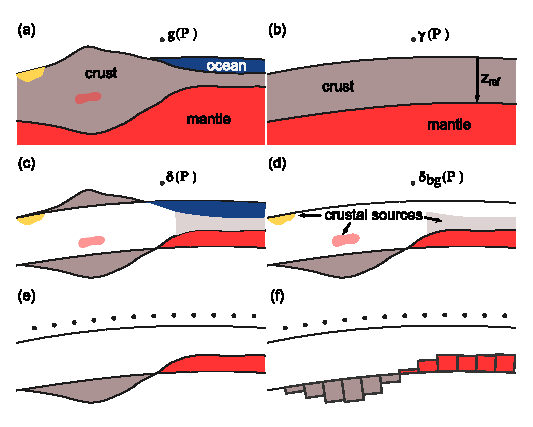
\includegraphics{figures/problem-concept}
    \caption{
        Sketch of the stages in gravity data correction and
        the discretization of the anomalous Moho relief using tesseroids.
        (a) The Earth and the measured gravity at point P ($g(P)$).
        (b) The Normal Earth and the calculated normal gravity at point P
        ($\gamma(P)$). $z_{ref}$ is the depth of the Normal Earth Moho.
        (c) The gravity disturbance ($\delta(P)$) and
        the corresponding density anomalies after removal of the normal gravity:
        topography, oceans, crustal heterogeneities, and the anomalous Moho.
        (d) The Bouguer disturbance ($\delta_{bg}(P)$) after topographic
        correction and the remaining density anomalies.
        (e) All density anomalies save the anomalous Moho are assumed to have
        been removed before inversion.
        (f) The discretization of the anomalous Moho in tesseroids. Grey
        tesseroids will have a negative density contrast while red tesseroids
        will have a positive one.
    }
    \label{fig:anomalysketch}
\end{figure}

\begin{figure}
    \centering
    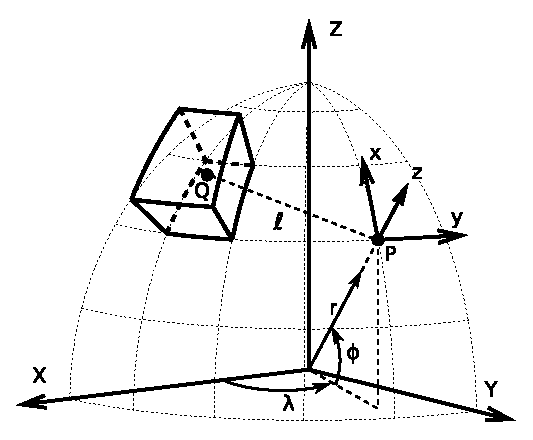
\includegraphics{figures/tesseroid-coord-sys}
    \caption{Sketch of a tesseroid (spherical prism) in a geocentric coordinate
        system (X, Y, Z).
        Observations are made at point P with respect to it's local
        North-oriented coordinate system (x, y, z).
        After \citet{uieda2015}.
    }
    \label{fig:tesseroid}
\end{figure}


In potential field methods,
we must isolate the target anomalous density distribution prior to modeling and
inversion.
In our case, the target is the relief of the real Moho undulating around a
reference Moho.
We do this by removing all other effects from the gravity observations.
The first correction is to remove the
scalar gravity of an ellipsoidal reference Earth (the Normal Earth),
hereafter denoted as $\gamma$.
This effect is calculated on the same point $P$ where
the gravity observation was made
(Fig~\ref{fig:anomalysketch}a-b).
$\gamma(P)$ is calculated using
the closed-form solution presented by \citet{li2001a}.
The difference between the observed gravity at point P ($g(P)$)
and Normal gravity at the same point
is known as the gravity disturbance,

\begin{equation}
    \delta(P) = g(P) - \gamma(P).
    \label{eq:disturbance}
\end{equation}

The disturbance contains only the gravitational effects of density
distributions that are anomalous with respect to the Normal Earth
(see Fig.~\ref{fig:anomalysketch}c).
This includes all masses above the surface of the ellipsoid (the topography),
the mass deficiency of the oceans,
the mass deficiency of sedimentary basins,
crustal sources (e.g., igneous intrusions, lateral density changes, etc),
heterogeneities below the upper mantle,
and the effect of the difference between the real Moho
topography and the Moho of the Normal Earth.

In order to invert for the anomalous Moho relief,
we must first isolate its gravitational attraction.
Thus, all other effects
must be either removed or assumed negligible.
Here, we will remove the effect of the topography and oceans
in order to obtain the full Bouguer disturbance
(Fig~\ref{fig:anomalysketch}d),

\begin{equation}
    \delta_{bg}(P) = \delta(P) - g_{topo}(P).
    \label{eq:bouguer}
\end{equation}

\noindent
We will remove the effect of sedimentary basins
but assume that the effects of
other crustal and mantle sources are negligible.
Thus, the only effect left will be that of the anomalous Moho relief
(Fig~\ref{fig:anomalysketch}e).
The gravitational attraction of the topography, oceans, and basins are
calculated in a spherical Earth approximation by forward modeling using
tesseroids (Fig.~\ref{fig:tesseroid}).
The tesseroid effects are calculated numerically using
Gauss-Legendre Quadrature (GLQ) integration \citep{asgharzadeh2007}.
The accuracy of the GLQ integration is improved by the adaptive discretization
scheme of \citet{uieda2016}.




%%%%%%%%%%%%%%%%%%%%%%%%%%%%%%%%%%%%%%%%%%%%%%%%%%%%%%%%%%%%%%%%%%%%%%%%%%%%%%%
\subsection{Parametrization}

We parameterize the forward problem by discretizing the anomalous Moho
into a grid of $M_{lon} \times M_{lat} = M$ juxtaposed tesseroids
(Fig~\ref{fig:anomalysketch}f).
The true (real Earth) Moho varies in depth
with respect to the Moho of the Normal Earth.
Hereafter we will refer to the depth of the Normal Earth Moho as $z_{ref}$
(see Fig.~\ref{fig:anomalysketch}b).
In cases where the true Moho is above $z_{ref}$,
the top of the $k$th tesseroid is the Moho depth $z_{k}$,
the bottom is $z_{ref}$, and the density-contrast ($\Delta\rho$) is positive
(red tesseroids in Fig~\ref{fig:anomalysketch}f).
If the Moho is below $z_{ref}$, the top of the tesseroid is $z_{ref}$,
the bottom is $z_k$, and $\Delta\rho$ is negative
(grey tesseroids in Fig~\ref{fig:anomalysketch}f).

Considering that the absolute value of the density-contrasts
of the tesseroids is a fixed parameter,
the predicted gravity anomaly of the Moho is a non-linear function of the
parameters $z_k$, $k=1, \ldots, M$,

\begin{equation}
    d_i = f_i(\mathbf{p}),
    \label{eq:forward}
\end{equation}

\noindent in which $d_i$ is the $i$th element of the $N$-dimensional predicted
data vector $\mathbf{d}$, $\mathbf{p}$ is the $M$-dimensional parameter vector
containing the $M$ Moho depths ($z_k$),
and $f_i$ is the $i$th non-linear function that maps the parameters onto the
data.
The functions $f_i$ are the radial component of the gravitational attraction
of the tesseroid Moho model.



%%%%%%%%%%%%%%%%%%%%%%%%%%%%%%%%%%%%%%%%%%%%%%%%%%%%%%%%%%%%%%%%%%%%%%%%%%%%%%%
\subsection{Inverse problem}

We wish to estimate the parameter vector $\mathbf{p}$ from a set of observed
gravity anomaly data $\mathbf{d}^o$.
The least-squares estimate is the one that minimizes the data-misfit function

\begin{equation}
    \phi(\mathbf{p}) =
    [\mathbf{d}^o - \mathbf{d}(\mathbf{p})]^T[\mathbf{d}^o - \mathbf{d}(\mathbf{p})].
    \label{eq:data-misfit}
\end{equation}

Function $\phi(\mathbf{p})$ is non-linear with respect to $\mathbf{p}$.
Thus, we can determine its minimum using gradient-based
iterative optimization
methods like Gauss-Newton or Steepest Descent.
Such methods start from an initial estimate $\mathbf{p}^0$ and iteratively
update the estimate until a minimum is reached.

For the Gauss-Newton method,
the update at the $k$th iteration,
$\mathbf{\Delta p} = \mathbf{p}^{k+1} - \mathbf{p}^k$,
is the solution of the linear system

\begin{equation}
    \mathbf{H}^k\mathbf{\Delta p} = -\mathbf{\nabla\phi}^k,
    \label{eq:gaussnewton}
\end{equation}

\noindent in which
$\mathbf{\nabla\phi}^k$ and $\mathbf{H}^k$ are, respectively,
the gradient vector and the Hessian matrix of $\phi(\mathbf{p})$.

The Steepest Descent method uses only the gradient direction
to update the initial estimate \citep{kelley1987}.
The update at the $k$th iteration is achieved by equating the Hessian
in Eq.~\ref{eq:gaussnewton} to the identity matrix,

\begin{equation}
    \mathbf{\Delta p} = -\mathbf{\nabla\phi}^k.
    \label{eq:steepest}
\end{equation}

\noindent
Thus, it does not require the computation and storage of the Hessian matrix
nor the solution of linear systems.
However, the Steepest Descent method has poor convergence when the
current solution is close to the minimum of the goal function
\citep{kelley1987}.

The gradient vector and the Gauss-Newton approximation of the Hessian matrix
of $\phi(\mathbf{p})$ are, respectively,

\begin{equation}
    \mathbf{\nabla\phi}^k = -2\mathbf{A}^T[\mathbf{d}^o - \mathbf{d}(\mathbf{p}^k)],
    \label{eq:gradient}
\end{equation}

\noindent
and

\begin{equation}
    \mathbf{H}^k \approx 2\mathbf{A}^T\mathbf{A},
    \label{eq:hessian}
\end{equation}

\noindent in which
$\mathbf{A}$ is the Jacobian or sensitivity matrix,

\begin{equation}
    A_{ij} = \dfrac{\partial f_i}{\partial p_j}(\mathbf{p^k}).
    \label{eq:jacobian}
\end{equation}



%%%%%%%%%%%%%%%%%%%%%%%%%%%%%%%%%%%%%%%%%%%%%%%%%%%%%%%%%%%%%%%%%%%%%%%%%%%%%%%
\subsection{Regularization}

Non-linear inversions for the relief of an interface (like the Moho)
are ill-posed and require additional constraints in the form of
regularization \citep{silva2001}.
A common approach is to use the first-order Tikhonov regularization to impose
smoothness on the solution.
The cost function for smoothness regularization is given by

\begin{equation}
    \theta(\mathbf{p}) = \mathbf{p}^T\mathbf{R}^T\mathbf{R}\mathbf{p},
    \label{eq:regul}
\end{equation}

\noindent where $\mathbf{R}$ is an $L \times M$ finite-difference matrix
representing the $L$ first-order differences between adjacent tesseroids.

The solution $\hat{\mathbf{p}}$ to the regularized inverse problem is the one that
minimizes the goal function

\begin{equation}
    \Gamma(\mathbf{p}) = \phi(\mathbf{p}) + \mu\theta(\mathbf{p}),
    \label{eq:goalfunction}
\end{equation}

\noindent
in which $\mu$ is the regularization parameter that controls the balance
between fitting the observed data and obeying the smoothness constraint.

The goal function $\Gamma(\mathbf{p})$ is also non-linear with respect to
$\mathbf{p}$ and can be minimized using the Gauss-Newton or Steepest Descent
methods.
The gradient vector and Hessian matrix of the goal function are, respectively,

\begin{equation}
    \mathbf{\nabla\Gamma}^k =
        -2\mathbf{A}^T[\mathbf{d}^o - \mathbf{d}(\mathbf{p}^k)] +
        2\mu\mathbf{R}^T\mathbf{R}\mathbf{p}^k,
    \label{eq:gradient-regul}
\end{equation}

\noindent and

\begin{equation}
    \mathbf{H}^k = 2\mathbf{A}^T\mathbf{A} + 2\mu\mathbf{R}^T\mathbf{R}.
    \label{eq:hessian-regul}
\end{equation}

\noindent The parameter updates for the regularized Gauss-Newton and Steepest
Descent methods, respectively, then become

\begin{equation}
    \left[\mathbf{A}^T\mathbf{A} + \mu\mathbf{R}^T\mathbf{R}\right]
    \mathbf{\Delta p} =
        \mathbf{A}^T[\mathbf{d}^o - \mathbf{d}(\mathbf{p}^k)] -
        \mu\mathbf{R}^T\mathbf{R}\mathbf{p}^k,
    \label{eq:gaussnewton-regul}
\end{equation}

\noindent and

\begin{equation}
    \mathbf{\Delta p} =
        \mathbf{A}^T[\mathbf{d}^o - \mathbf{d}(\mathbf{p}^k)] -
        \mu\mathbf{R}^T\mathbf{R}\mathbf{p}^k,
    \label{eq:steepest-regul}
\end{equation}

Producing the regularized solution using the above equations is computationally
costly because of two main factors:
(1) the evaluation and storage of the dense $N \times M$ Jacobian matrix
$\mathbf{A}$
and (2) the solution of the resulting $M \times M$ equation system
(not required for Steepest Descent).
In practice, the derivatives in the Jacobian (Eq.~\ref{eq:jacobian})
are often calculated through a first-order finite-difference approximation.
Thus, evaluating $\mathbf{A}$ requires $2\times M \times N$ forward modeling
operations for each iteration of the gradient descent algorithm.
These computations are performed for each iteration of the optimization.


%%%%%%%%%%%%%%%%%%%%%%%%%%%%%%%%%%%%%%%%%%%%%%%%%%%%%%%%%%%%%%%%%%%%%%%%%%%%%%%
\subsection{Bott's method}

\citet{bott1960} developed an efficient method to determined the basement
relief of a sedimentary basin from gravity observations.
The method requires data on a regular grid of $N_x \times N_y = N$
observations.
The basement relief is then discretized into an equal grid of $M_x \times
M_y = M$ elements with $M_x = N_x$ and $M_y = N_y$.
Bott's iterative method starts with an initial estimate of the basement relief
$\mathbf{p}^0$ equal to the null vector and updates the estimate using the formula

\begin{equation}
    \mathbf{\Delta p} = \dfrac{\mathbf{d}^o - \mathbf{d}(\mathbf{p}^k)}{2\pi G \Delta \rho},
    \label{eq:bott}
\end{equation}

\noindent
in which $G$ is the gravitational constant and $\Delta \rho$ is the basin
density contrast.
The iterative process stops when the inversion residuals
$\mathbf{r} = \mathbf{d}^o - \mathbf{d}(\mathbf{p}^k)$ fall below the assumed noise level
of the data.

\citet{silva2014} showed that Bott's method can be formulated as
a special case of the Gauss-Newton method (Eq.~\ref{eq:gaussnewton})
by setting the Jacobian matrix (Eq.~\ref{eq:jacobian}) to

\begin{equation}
    \mathbf{A} = 2\pi G \Delta \rho \mathbf{I},
    \label{eq:bott-gaussnewton}
\end{equation}

\noindent
in which $\mathbf{I}$ is the identity matrix.
In this framework,
Bott's method uses a Bouguer plate approximation of the gravitational effect of
the relief, $d_i = 2\pi G \Delta\rho z_i$.
The derivative of $d_i$ with respect to the parameter $z_i$ is
$2\pi G \Delta \rho$, thus linearizing the Jacobian matrix.
However, the non-linearity of the predicted data $\mathbf{d}(\mathbf{p}^k)$ is
preserved.

We propose that Bott's method can also be formulated as a special case of the
Steepest Descent method (Eq.~\ref{eq:steepest}) by setting the Jacobian matrix to

\begin{equation}
    \mathbf{A} = \dfrac{1}{4 \pi G \Delta \rho}\mathbf{I}.
    \label{eq:bott-steepest}
\end{equation}

\noindent
In practice, both formulations lead to Eq.~\ref{eq:bott}.
One of the advantages of Bott's method over the traditional Gauss-Newton or
Steepest Descent is eliminating the computation and storage of the dense
Jacobian matrix $\mathbf{A}$.
Furthermore, Bott's method also does not require the solution of equation
systems.
However, a disadvantage of Bott's method is that it suffers from instability
\citep{silva2014}.
A common approach to counter this issue is to apply a smoothing filter after
the inversion to the unstable estimate, as in \citet{silva2014}.



%%%%%%%%%%%%%%%%%%%%%%%%%%%%%%%%%%%%%%%%%%%%%%%%%%%%%%%%%%%%%%%%%%%%%%%%%%%%%%%
\subsection{Regularized Bott's method in spherical coordinates}

We propose a regularized version of Bott's method to invert for the relief of
the anomalous Moho in spherical coordinates.
To adapt Bott's method to spherical coordinates,
we replace the right-rectangular prisms in the forward modeling
($\mathbf{d}(\mathbf{p}^k)$ in Eq.~\ref{eq:bott})
with tesseroids.
The tesseroid forward modeling uses the adaptive discretization algorithm
of \citet{uieda2016} to achieve accurate results.
Furthermore, our formulation maintains the regularized solution
for the Gauss-Newton method (Eq.~\ref{eq:gaussnewton-regul})
but replaces the full Jacobian matrix with the Bouguer plate approximation
(Eq.~\ref{eq:bott-gaussnewton}).
This linearizes the Jacobian matrix and reduces it to a sparse diagonal matrix,
thus eliminating the cost of computing and storing $\mathbf{A}$.
Matrix arithmetic operations can be performed efficiently by taking advantage
of the sparse nature of matrices $\mathbf{A}$ and $\mathbf{R}$
(respectively, Eq.~\ref{eq:bott-gaussnewton} and \ref{eq:regul}).
The same is true for solving the equation system in the Gauss-Newton method
(Eq.~\ref{eq:gaussnewton-regul}).
However, the computational cost of forward modeling is still present.
Particularly, forward modeling using tesseroids is more computationally
intensive than using right-rectangular prisms
because of the numerical integration and adaptive discretization
\citep{uieda2016}.
Our benchmarks suggest that
sparse matrix multiplications and solving the sparse linear system
in Eq.~\ref{eq:gaussnewton-regul}
account for less than 0.1\%
of the computation time of a single inversion
(see section~\ref{sec:simple-synthetic} and table~\ref{profiling}).
Hence, by employing the use of sparse matrices,
our formulation retains the efficiency of Bott's method
while stabilizing the solution through the well established formalism of
Tikhonov regularization.



%%%%%%%%%%%%%%%%%%%%%%%%%%%%%%%%%%%%%%%%%%%%%%%%%%%%%%%%%%%%%%%%%%%%%%%%%%%%%%%
\subsection{Estimating the regularization parameter}

\begin{figure}
    \centering
    \includegraphics{figures/cv-grid-separation}
    \caption{Sketch of a data grid separated into
        the training (white dots with black outlines)
        and testing (black dots) data sets.
        The training data set is still displayed on a regular grid
        but with twice the grid spacing
        of the original data grid.}
    \label{fig:grid_separation}
\end{figure}

The regularization parameter $\mu$ controls how much smoothness is applied to
the inversion result.
An optimal value of $\mu$ will stabilize and smooth the solution while not
compromising the fit to the observed data.
Two widely used methods to estimate an optimal $\mu$ are
the L-curve criterion and cross-validation \citep{hansen1992}.
Here, we will adopt the hold-out method of cross-validation \citep{kim2009}.
The hold-out method consists of splitting the observed data set into two
independent parts:
a training set $\mathbf{d}^o_{inv}$
and a testing set $\mathbf{d}^o_{test}$.
The training set is used in the inversion
while the testing set is kept back
and used to judge the quality of the chosen value of $\mu$.
For a value of the regularization parameter $\mu_k$,
the training set is inverted using $\mu_k$
to obtain an estimate $\mathbf{\hat{p}}^k$.
This estimate is used to calculate predicted data
on the same points as the testing set
via forward modeling
($\mathbf{d}_{test}^k = \mathbf{f}(\mathbf{\hat{p}}^k$)).
The metric chosen to evaluate $\mu_k$ is
the mean square error (MSE) of the misfit
between the observed and predicted testing data sets,

\begin{equation}
    MSE_k = \dfrac{\|\mathbf{d}^o_{test} - \mathbf{d}^k_{test}\|^2}{N_{test}},
    \label{eq:msemu}
\end{equation}

\noindent
in which $N_{test}$ is the number of data in the testing set.
The optimal value of $\mu$ will be the one that minimizes the MSE,
i.e. the one that best predicts the testing data.
We emphasize that the inversion is performed only on the training data set.

The algorithm for the hold-out cross-validation is summarized as follows:

\begin{enumerate}
    \item Divide the observed data into
        the training ($\mathbf{d}^o_{inv}$)
        and testing ($\mathbf{d}^o_{test}$) sets.
    \item For each $\mu_k \in [\mu_1, \mu_2, \ldots, \mu_{N_{\mu}}]$:
    \begin{enumerate}
        \item Estimate $\mathbf{\hat{p}}^k$ by inverting the training set
            $\mathbf{d}^o_{inv}$.
        \item Use $\mathbf{\hat{p}}^k$ to calculate the predicted testing set
            $\mathbf{d}^k_{test}$.
        \item Calculate the mean square error $MSE_k$ using Eq.~\ref{eq:msemu}.
    \end{enumerate}
    \item The final solution is the $\mathbf{\hat{p}}^k$ corresponding to the
        smallest $MSE_k$.
\end{enumerate}

The separation of the training and testing data sets is commonly done by taking
random samples from the full data set.
However, we cannot perform the separation in this way because
Bott's method requires data on a regular grid as well as having model elements
directly below each data point.
Thus, we take as our training set the points from the observed data grid that
fall on a similar grid but with twice the grid spacing
(white dots with black outlines in Fig.~\ref{fig:grid_separation}).
All other points from the original data grid
make up the testing data set
(black dots in Fig.~\ref{fig:grid_separation}).
This separation will lead to
a testing data set with more points than the training data set.
A way to balance this loss of data in the inversion
is to generate a data grid with half of the desired grid spacing,
either through interpolation
or from a spherical harmonic model.



%%%%%%%%%%%%%%%%%%%%%%%%%%%%%%%%%%%%%%%%%%%%%%%%%%%%%%%%%%%%%%%%%%%%%%%%%%%%%%%
\subsection{Estimating $z_{ref}$ and $\Delta\rho$}

The depth of the Normal Earth Moho ($z_{ref}$)
and the density-contrast of the anomalous Moho ($\Delta\rho$)
are other hyper-parameters of the inversion.
That is, their value influences the final solution
but they are not estimated during the inversion.
Both hyper-parameters cannot be determined from the gravity data alone.
Estimating $z_{ref}$ and $\Delta\rho$ requires
information that is independent of the gravity data,
such as knowledge of the parameters at certain points.
This information can be used in a manner similar to
the cross-validation described in the previous section.
In this study, we use point estimates of the Moho depth
to determine the optimal values of $z_{ref}$ and $\Delta\rho$.
These points will generally come from seismologic studies,
like receiver functions, surface wave dispersion, and deep refraction
experiments.

Let $\mathbf{z}_s^o$ be a vector of $N_s$ known Moho depths.
We use the mean square error (MSE)
as a measure of how well a given inversion output $\mathbf{\hat{p}}^k$
fits the know depths.
The optimal values of $z_{ref}$ and $\Delta\rho$
are the ones that best fit the independent known Moho depths
(i.e., produce the smallest MSE).
However, the points do not necessarily coincide
with the model elements of the inversion.
Before computing the MSE,
we interpolate $\mathbf{\hat{p}}^k$ on the known points
to obtain the predicted depths $\mathbf{z}_s^k$.
The MSE is defined as

\begin{equation}
    MSE = \dfrac{\|\mathbf{z}^o_s - \mathbf{z}^k_{s}\|^2}{N_s}.
    \label{eq:msehyper}
\end{equation}

The algorithm for estimating $z_{ref}$ and $\Delta\rho$ is:

\begin{enumerate}
    \item For every combination of
        $z_{ref,l} \in [z_{ref,1},z_{ref,2},\ldots,z_{ref,N_z}]$ and
        $\Delta\rho_m \in
         [\Delta\rho_1,\Delta\rho_2,\ldots,\Delta\rho_{N_{\rho}}]$:
    \begin{enumerate}
        \item Perform the inversion on the training data set
            $\mathbf{d}^o_{inv}$ using $z_{ref,l}$, $\Delta\rho_m$, and
            the previously estimated value of $\mu$.
            The inversion output is the vector $\mathbf{\hat{p}}^{l,m}$.
        \item Interpolate $\mathbf{\hat{p}}^{l,m}$
            on the known points to obtain the predicted depths
            $\mathbf{z}_s^{l,m}$.
        \item Calculate the MSE between $\mathbf{z}_s^o$ and
            $\mathbf{z}_s^{l,m}$ using Eq.~\ref{eq:msehyper}.
    \end{enumerate}
    \item The final solution is the $\mathbf{\hat{p}}^{l,m}$ corresponding to
        the smallest MSE.
\end{enumerate}

A similar approach was used by \citet{martins2010}
to estimate the parameters defining
the density-contrast variation with depth
of a sedimentary basin.
\citet{vandermeijde2013} also had
a similar methodology for dealing with the hyper-parameters,
though in a less formalized way.



%%%%%%%%%%%%%%%%%%%%%%%%%%%%%%%%%%%%%%%%%%%%%%%%%%%%%%%%%%%%%%%%%%%%%%%%%%%%%%%
\subsection{Software implementation}

The inversion method proposed here is implemented in the Python programming
language.
The software is freely available
under the terms of the BSD 3-clause open-source software license.
Our implementation relies on the open-source libraries
scipy and numpy \citep[][ \url{http://scipy.org}]{jones2001}
for array-based computations,
matplotlib \citep[][ \url{http://matplotlib.org}]{hunter2007}
and seaborn
\citep[][ \url{http://stanford.edu/~mwaskom/software/seaborn}]{waskom2015}
for plots and maps,
and Fatiando a Terra \citep[][ \url{http://www.fatiando.org}]{uieda2013}
for geophysics specific tasks,
particularly for forward modeling using tesseroids.
We use the scipy.sparse package for sparse matrix arithmetic and linear
algebra.
The sparse linear system in Eq.~\ref{eq:gaussnewton-regul}
is solved using the conjugate gradient method implemented in scipy.sparse.

The computational experiments
(e.g., data processing, synthetic tests, real data application)
were performed in
Jupyter (formerly IPython) notebooks
\citep[][ \url{http://jupyter.org/}]{perez2007}.
The notebook files combine the source code used to run the experiments,
the results and figures generated by the code,
and rich text to explain and document the analysis.

All source code, data, and Jupyter notebooks
can be found at the online repository
\url{https://github.com/pinga-lab/paper-moho-inversion-tesseroids}.
The repository also contains instructions for replicating all results presented
here.
An archived version of this repository is also available at
\url{http://dx.doi.org/...}
(\textbf{Note to reviewers: the archived version will be uploaded only upon
publication}).


%%%%%%%%%%%%%%%%%%%%%%%%%%%%%%%%%%%%%%%%%%%%%%%%%%%%%%%%%%%%%%%%%%%%%%%%%%%%%%%
\section{Application to synthetic data}

We test and illustrate the proposed inversion method
by applying it to two noise-corrupted synthetic data sets.
The first data set is generated by a simple Moho model simulating the transition
from a thicker continental crust to a thinner oceanic crust.
This application uses cross-validation to estimate the regularizing parameter
($\mu$) while assuming that the anomalous Moho density-contrast ($\Delta\rho$)
and the Normal Earth Moho depth ($z_{ref}$) are known quantities.
This first test is simplified in order to investigate solely
the efficiency of the inversion and
the cross-validation procedure to estimate $\mu$.
The second data set is generated by a more complex model derived from
the South American portion of the global CRUST1.0 model \citep{laske2013}.
This application uses cross-validation to estimate all three hyper-parameters:
$\mu$, $\Delta\rho$, and $z_{ref}$.
The model and corresponding synthetic data are meant to simulate
with more fidelity the real data application.


%%%%%%%%%%%%%%%%%%%%%%%%%%%%%%%%%%%%%%%%%%%%%%%%%%%%%%%%%%%%%%%%%%%%%%%%%%%%%%%
\subsection{Simple model}\label{sec:simple-synthetic}

\begin{figure}
    \centering
    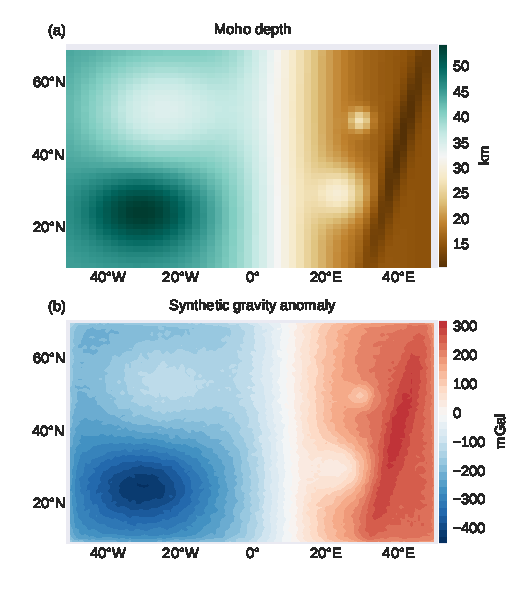
\includegraphics{figures/synthetic-simple-data}
    \caption{
        A simple Moho model made of tesseroids for synthetic data application.
        (a) The Moho depth of the model in kilometers.
        The model transitions from a deep Moho in the right to a shallow Moho in
        left, simulating the transition between a continental and an oceanic
        Moho.
        Each pixel in the pseudo-color image corresponds to a tesseroid of the
        model.
        (b) Noise-corrupted synthetic gravity data generated from the model
        shown in (a).
    }
    \label{fig:simple-data}
\end{figure}

\begin{figure*}
    \centering
    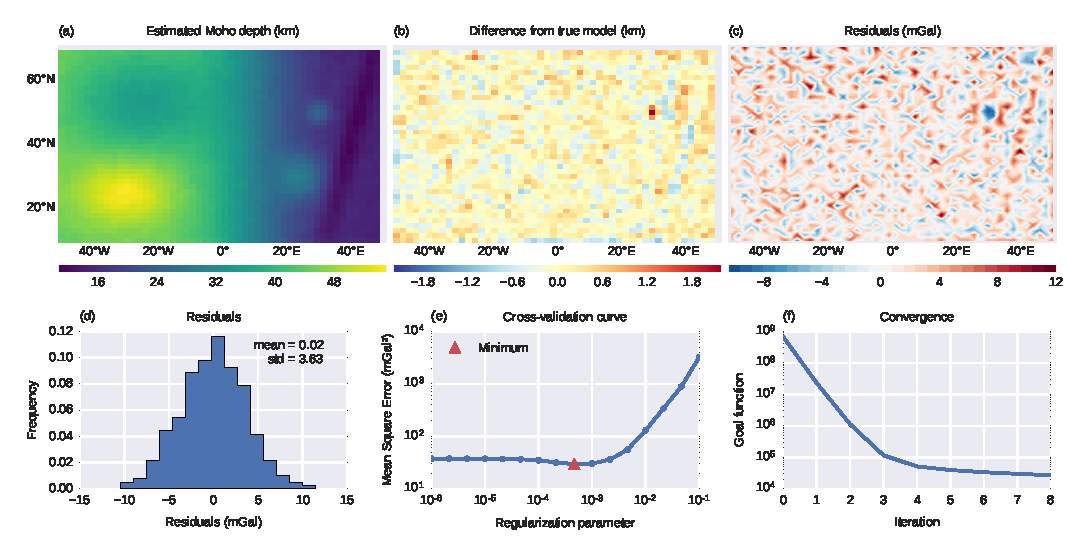
\includegraphics[width=\textwidth]{figures/synthetic-simple-results}
    \caption{
        Results from the inversion of the simple synthetic data.
        (a) The estimated Moho depth.
        (b) The difference between the true model depths
        and the estimated depths.
        (c) The inversion residuals (observed data minus
        the data predicted by the estimate).
        (d) Histogram of the residuals. Also shown are the calculated
        mean and standard deviation (std) of the residuals.
        Note that the data were contaminated with normally distributed
        pseudo-random noise with zero mean and 5 mGal standard deviation.
        (e) Cross-validation curve used to determine the optimal regularization
        parameter (Eq.~\ref{eq:goalfunction}).
        Both axis are in logarithmic scale.
        The minimum Mean Square Error (Eq.~\ref{eq:msemu}) is found at
        $\mu = 0.00046$ (red triangle).
        (f) Goal function value (Eq.~\ref{eq:goalfunction}) per Gauss-Newton
        iteration showing the convergence of the gradient descent.
        The y-axis is in logarithmic scale.
    }
    \label{fig:simple-results}
\end{figure*}

We simulate the transition from a continental-type Moho to an oceanic-type Moho
using a model composed of $M_{lat} \times M_{lon} = 40 \times 50$ grid of
juxtaposed tesseroids (a total of $M = 2000$ model elements).
The anomalous Moho density-contrast is $\Delta\rho = 400\ kg/m^3$
and the Normal Earth Moho depth is $z_{ref} = 30\ km$.
Fig.~\ref{fig:simple-data}a shows the model Moho depths,
where each pixel in the pseudo-color image corresponds to
a tesseroid of the model.

The synthetic data were forward modeled on a regular grid of
$N_{lat} \times N_{lon} = 79 \times 99$ points
(a total of $N = 7821$ observations)
at a constant height of 50 km.
The data were contaminated with pseudo-random noise
sampled from a normal distribution with zero mean and 5 mGal standard deviation.
Fig.~\ref{fig:simple-data}b shows the noise-corrupted full synthetic data set.
The data grid spacing is half the grid spacing of the tesseroid model
so that, when separating the training and testing data sets
(Fig.~\ref{fig:grid_separation}),
the training data set points will fall directly above each model element.

We separated the synthetic data into training and testing data sets
following Fig.~\ref{fig:grid_separation}.
The training data set is a regular grid of
$N_{lat} \times N_{lon} = 40 \times 50$ points
(a total of $N_{train} = 2000$).
The testing data set is composed of $N_{test} = 5821$ observations.
We used cross-validation to estimate an optimal regularization parameter ($\mu$)
from a set of $N_\mu = 16$ values equally spaced on a logarithmic scale
between $10^{-6}$ and $10^{-1}$.
We ran our regularized inversion on the training data set
for each value of $\mu$,
obtaining 16 Moho depth estimates.
For all inversions, the initial Moho depth estimate
used to start the Gauss-Newton optimization
was set to 60 km depth for all inversion parameters.
Furthermore, $z_{ref}$ and $\Delta\rho$ are set to their respective true values.
Finally, we computed the mean square error (MSE, Eq.~\ref{eq:msemu})
for each estimate and chose as the final estimated Moho model
the one that minimizes the MSE.

Fig.~\ref{fig:simple-results} summarizes the inversion results.
Fig.~\ref{fig:simple-results}a shows the final estimated Moho depth
after cross-validation.
The recovered model is smooth, indicating that the cross-validation procedure
was effective in estimating an optimal regularization parameter.
Fig.~\ref{fig:simple-results}b shows difference between the true Moho depth
(Fig.~\ref{fig:simple-data}a) and the estimated Moho depth.
The differences appear to be semi-randomly distributed with a maximum
coinciding with a short-wavelength feature in the true model.
The maximum and minimum differences are approximately
2.19 and -2.13 km, respectively.
Fig.~\ref{fig:simple-results}c shows inversion residuals (difference between
the observed and predicted data), in mGal.
The largest residual (in absolute value) coincides with the largest difference
between the true model and the estimate.
The inversion residuals are normally distributed,
as shown in Fig.~\ref{fig:simple-results}d,
with 0.02 mGal mean and a standard deviation of 3.63 mGal.
The cross-validation curve in Fig.~\ref{fig:simple-results}e
shows a clear minimum MSE at $\mu = 0.00046$
(indicated by the red triangle).
Fig.~\ref{fig:simple-results}f shows the convergence of
the Gauss-Newton optimization in eight iterations.

We also investigated the computation time spent in each section of the inversion
process using a source code profiler.
The profiler measures how much time is spent inside each function during
the execution of a program.
We ran the profiler on a single inversion of the training data set
using the estimated regularization parameter.
We tracked the total time spent inside each of the three functions
that represent the largest computational bottlenecks of the inversion:
solving the linear system in Eq.~\ref{eq:gaussnewton-regul}
using the conjugate gradient method,
performing the dot products required to compute
the Hessian matrix (Eq.~\ref{eq:hessian-regul})
and the gradient vector (Eq.~\ref{eq:gradient-regul}),
and forward modeling to calculate the predicted data (Eq.~\ref{eq:forward}).
The profiling results presented in table~\ref{profiling}
show that the time spent on forward modeling accounts for approximately
99.8\% of the total computation time.


% Insert the profiling results table

\begin{table}
    \centering
    \caption{
        Time spent on each function during a single inversion of
        simple synthetic data.
        The inversion was performed on a laptop computer with a
        Intel(R) Core(TM) i7-3612QM CPU @ 2.10GHz processor.
        The total time for the inversion was 42.133 seconds.
    }
    \label{profiling}
    \begin{tabular}{lcc}
        Function description & Time (s) & Percentage of total time (\%)\\
        \hline
        Sparse conjugate gradient & 0.021 & 0.050\\
        Sparse dot product & 0.007 & 0.017\\
        Tesseroid forward modeling & 42.059 & 99.824\\
        \hline
    \end{tabular}
\end{table}





%%%%%%%%%%%%%%%%%%%%%%%%%%%%%%%%%%%%%%%%%%%%%%%%%%%%%%%%%%%%%%%%%%%%%%%%%%%%%%%
\subsection{Model based on CRUST1.0}

\begin{figure*}
    \centering
    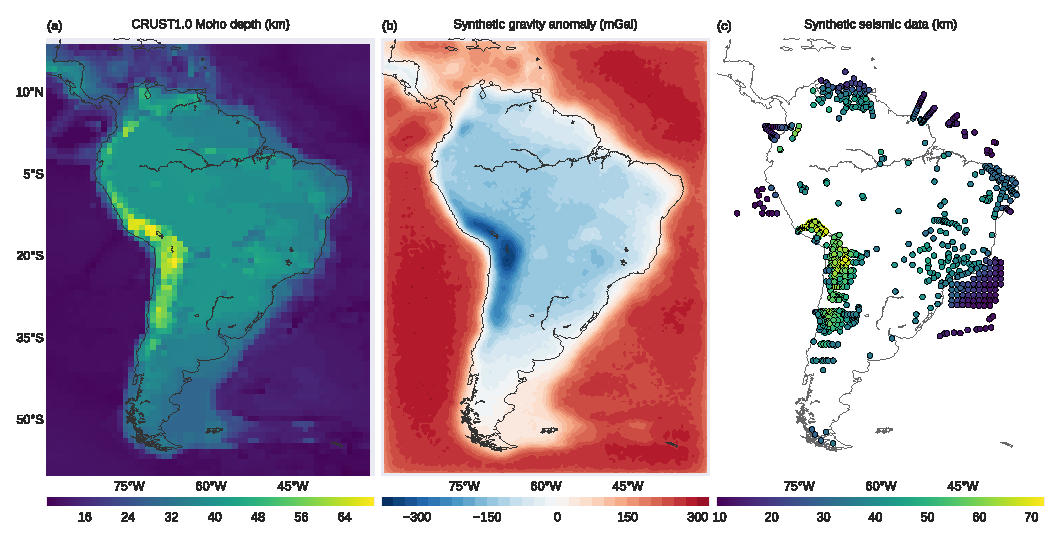
\includegraphics[width=\textwidth]{figures/synthetic-crust1-data}
    \caption{
        Synthetic data of a model derived from CRUST1.0.
        The model is made of tesseroids with an constant density-contrast
        of $\Delta\rho = 350\ kg/m^3$ and assuming a reference level of
        $z_{ref} = 30\ km$.
        (a) The Moho depth of the model in kilometers.
        Each pixel in the pseudo-color image corresponds to a tesseroid of the
        model.
        (b) Noise-corrupted synthetic gravity data generated from the model.
        (c) Synthetic seismic data simulating point estimates of Moho depth.
        The point estimates were obtained by interpolating
        the Moho depth in (a).
    }
    \label{fig:crust1-data}
\end{figure*}

\begin{figure*}
    \centering
    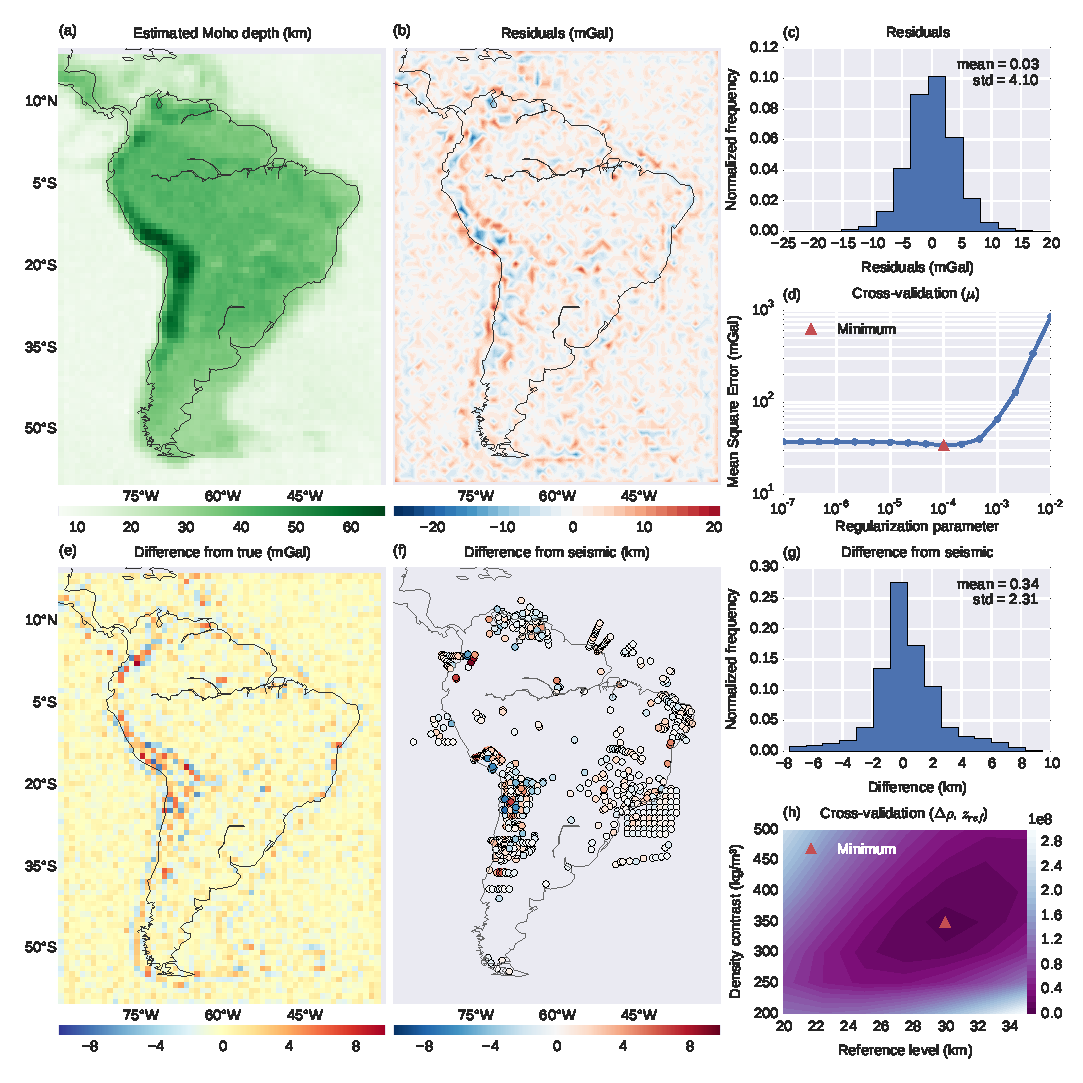
\includegraphics[width=\textwidth]{figures/synthetic-crust1-results}
    \caption{
        Inversion results from the CRUST1.0 synthetic data.
        (a) Cross-validation curve used to determine
        the regularization parameter (Eq.~\ref{eq:goalfunction}).
        The minimum Mean Square Error (Eq.~\ref{eq:msemu}) is found at
        $\mu = 0.0001$ (red triangle).
        (b) Cross-validation results used to determine
        the reference level ($z_{ref}$) and the density-contrast ($\Delta\rho$).
        The colored contours represent
        the Mean Square Error (Eq.~\ref{eq:msehyper}) in $km^2$.
        The minimum (red triangle) is found at $z_{ref} = 30\ km$
        and $\Delta\rho = 350\ kg/m^3$.
        (c) The estimated Moho depth.
        (d) Difference between the CRUST1.0 model depths
        (Fig.~\ref{fig:crust1-data}a)
        and the estimated depths.
        (e) Histogram of the inversion residuals
        (observed minus predicted data).
        (f) Histogram of the differences between
        the synthetic seismic observations (Fig.~\ref{fig:crust1-data}c)
        and the estimated depths.
        (g) The inversion residuals.
        (h) Difference between the seismic and the estimated depths.
    }
    \label{fig:crust1-results}
\end{figure*}


In this test, we simulate the anomalous Moho of South America
using Moho depth information extracted from the CRUST1.0 model
\citep{laske2013}.
We construct a tesseroid model with
$M_{lat} \times M_{lon} = 80 \times 60$ juxtaposed elements, 4800 in total,
using the Moho depths shown in Fig.~\ref{fig:crust1-data}a.
In our model, the Normal Earth Moho is $z_{ref} = 30\ km$ and
the density-contrast is $\Delta\rho = 350\ kg/m^3$.
We produce the synthetic data at a constant height of 50 km
and on a regular grid of $N_{lat} \times N_{lon} = 159 \times 119$ points
(a total of 18921 observations).
We contaminate the synthetic data with normally distributed pseudo-random noise
with zero mean and 5 mGal standard deviation (Fig.~\ref{fig:crust1-data}b).

The cross-validation procedure to determine $\Delta\rho$ and $z_{ref}$
requires knowledge of the Moho depth at certain points
($\mathbf{z}_s^o$ in Eq.~\ref{eq:msehyper}),
usually from seismic experiments.
Thus, we must also generate synthetic seismic data about the Moho depth.
We produce such data by interpolating the Moho depth shown in
Fig.~\ref{fig:crust1-data}a on the same geographic coordinates
as the 937 points from the \citet{assumpcao2012} data set.
The resulting synthetic seismic data is shown in Fig.~\ref{fig:crust1-data}c.

We perform the cross-validation procedures in two parts.
First, we run the cross-validation to estimate
an optimal regularization parameter ($\mu$).
The starting estimate for all inversions is
60 km depth for all model parameters.
For this cross-validation,
we keep $z_{ref}$ and $\Delta\rho$ fixed to
$20\ km$ and $500\ kg/m^3$, respectively.
Our investigations suggest that the outcome of this round of cross-validation
does not depend on the particular values of $z_{ref}$ and $\Delta\rho$ used.
Second, we use the estimated $\mu$ to run the cross-validation
to estimate $z_{ref}$ and $\Delta\rho$,
thus obtaining the final estimated Moho depths.
Fig.~\ref{fig:crust1-results} summarizes the results
from both cross-validation runs and the final inversion results.

For the first cross-validation,
we separate the synthetic data (Fig.~\ref{fig:grid_separation}) into
a training set with half the grid spacing of the original data
($N_{lat} \times N_{lon} = 80 \times 60$)
and a testing set with 14,121 observations.
We run the inversion for 16 different values of $\mu$
equally spaced in a logarithmic scale between $10^{-7}$ and $10^{-2}$.
For each of the 16 estimates we compute the MSE (Eq.~\ref{eq:msemu}),
shown in Fig.~\ref{fig:crust1-results}a as function of $\mu$.
The optimal regularization parameter that minimizes the MSE is $\mu = 10^{-4}$
(indicated by the red triangle).

In the second cross-validation,
we use the estimated value of $\mu$ in all inversions.
We test 7 values of $z_{ref}$ from 20 to 35 km with 2.5 km intervals
and 7 values of $\Delta\rho$ from 200 to 500 $kg/m^3$
with 50 $kg/m^3$ intervals.
We run the inversion for every combination of $z_{ref}$ and $\Delta\rho$,
totaling 49 inversions.
Finally, we calculate the Mean Square Error (Eq.~\ref{eq:msehyper})
for each of the 49 estimates
and choose the values of $z_{ref}$ and $\Delta\rho$ that minimize the MSE.
Fig.~\ref{fig:crust1-results}b
shows a colored-contour map of the MSE
with a minimum (marked by the red triangle)
at $z_{ref} = 30\ km$ and $\Delta\rho = 350\ kg/m^3$.

Fig.~\ref{fig:crust1-results}c shows the final solution after both
cross-validation procedures.
The recovered model is smooth, indicating that the cross-validation procedure
was effective in estimating an optimal regularization parameter.
Fig.~\ref{fig:crust1-results}d shows the difference between
the true Moho depths (Fig.~\ref{fig:crust1-data}a)
and the estimated depths.
The maximum and minimum differences are, respectively,
9.8 and -8.2 km.
The largest absolute differences are located along the central and northern
Andes, where there is a sharp increase in the true Moho depth
(Fig.~\ref{fig:crust1-data}a).
Positive differences (indicating a too shallow estimate)
appear along the central portion of the Andes,
flanked by regions of negative differences (indicating a too deep estimate)
on the continental and Pacific sides.
Figs.~\ref{fig:crust1-results}e and g show the inversion residuals (difference
between the observed and predicted data).
The inversion residuals appear normally distributed,
with 0.03 mGal mean and a standard deviation of 4.10 mGal.
The residuals follow a similar, though reversed, pattern
to the differences shown in Fig.~\ref{fig:crust1-results}d.
The largest residuals (in absolute value) are along the Andes,
with the central portion being dominated by negative residuals
and flanked by positive residuals on both sides.
Figs.~\ref{fig:crust1-results}f and h show the differences between
the synthetic seismic data (Fig.~\ref{fig:crust1-data}c)
and the estimated Moho depths.
Once more, the largest differences are concentrated along the Andes,
particularly in the central Andes and near Ecuador and Colombia.
The differences are smaller along the Atlantic coast of South America,
with notable larger differences in a few points of northeastern Brazil
and along the Amazon river.




%%%%%%%%%%%%%%%%%%%%%%%%%%%%%%%%%%%%%%%%%%%%%%%%%%%%%%%%%%%%%%%%%%%%%%%%%%%%%%%
\section{Application to the South American Moho}


We apply the inversion method proposed here to invert for the Moho depth of the
South American continent.
We follow the application of \citet{vandermeijde2013} but with some
differences, mainly using a different data set and performing all modeling
in spherical coordinates using tesseroids.
The data are corrected of the effects of topography and sedimentary basins.
Crust and mantle heterogeneities cannot be properly accounted for
in regions where information coverage is sparse and readily accessible models
are not available, like in South America and Africa.
Hence, for the purposes of this study, we will assume to be negligible all
other crustal and mantle sources, including lateral variations in density along
the Moho.


%%%%%%%%%%%%%%%%%%%%%%%%%%%%%%%%%%%%%%%%%%%%%%%%%%%%%%%%%%%%%%%%%%%%%%%%%%%%%%%
\subsection{Gravity and seismic data}

\begin{figure*}
    \centering
    \includegraphics[width=\textwidth]{figures/south-america-corrections}
    \caption{
        Gravity data for South America and the models used in the data
        corrections.
        (a) The gravity disturbance (Eq.~\ref{eq:disturbance}) calculated from
        the raw gravity data.
        (b) Topography from ETOPO1.
        (c) Gravitational attraction of the topography calculated
        at the observation height using tesseroids.
        (d) The Bouguer disturbance (Eq.~\ref{eq:bouguer}) obtained by
        subtracting (c) from (a).
        The upper (e), middle (f), and lower (g) sediment layer thicknesses
        from the CRUST1.0 model.
        (h) The total gravitational attraction of the sediment layers shown in
        (e), (f), and (g), calculated using tesseroids.
        }
    \label{fig:sam-corrections}
\end{figure*}

\begin{figure*}
    \centering
    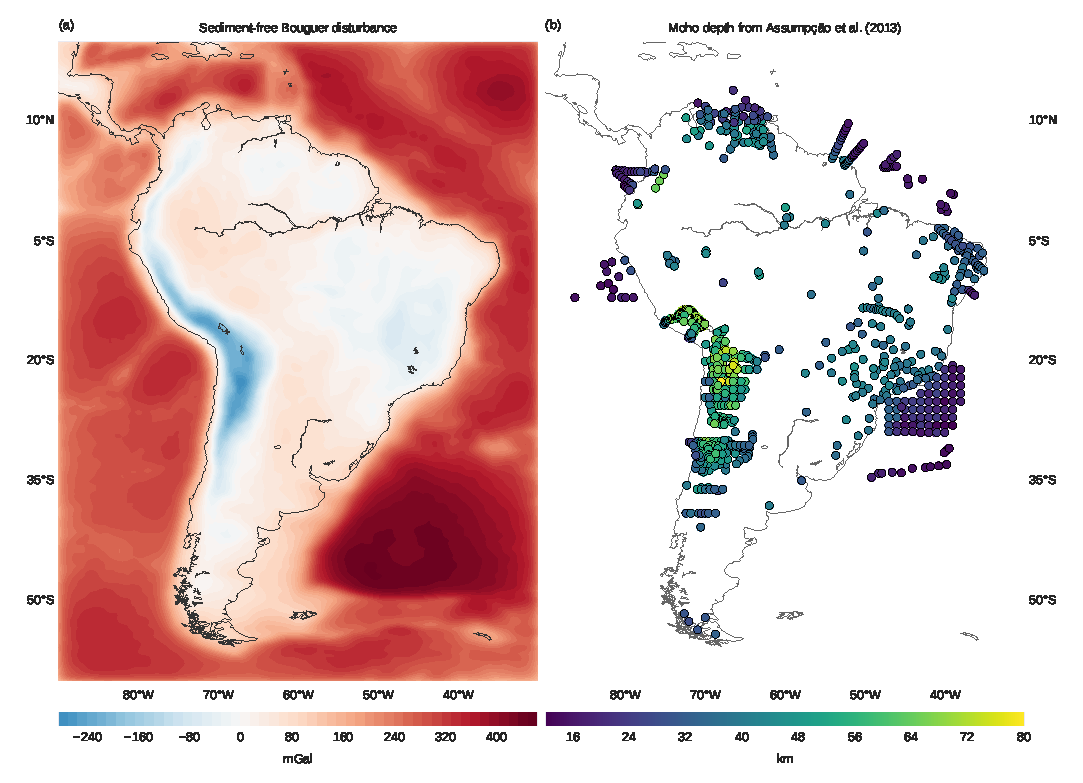
\includegraphics[width=\textwidth]{figures/south-america-data}
    \caption{
        Input data for the South American Moho inversion.
        (a) Sediment-free Bouguer disturbance for South America.
        Obtained by subtracting the total sediment gravitational effect
        (Fig.~\ref{fig:sam-corrections}h) from the Bouguer disturbance
        (Fig.~\ref{fig:sam-corrections}d).
        (b) Seismological Moho depth estimates from
        \citet{assumpcao2012}.
    }
    \label{fig:sam-data}
\end{figure*}


The raw gravity data are generated from the satellite only
spherical harmonic model GOCO5S \citet{mayer-guerr2015}.
The GOCO5S model combines data from 15 satellites, including the complete
mission data from the GOCE satellite.
The data were downloaded from the ICGEM web-service
(\url{http://icgem.gfz-potsdam.de/ICGEM/})
in the form of the complete gravity field
on a regular grid with $0.2^\circ$ grid spacing at ellipsoidal height 50 km.
We calculate the gravity disturbance
($\delta(P)$ in Eq.~\ref{eq:disturbance})
by subtracting from the raw data
the normal gravity of the WGS84 reference ellipsoid ($\gamma(P)$)
using the formula of \citet{li2001a}.
Fig.~\ref{fig:sam-corrections}a show the calculated gravity disturbance of
South America.

We remove the gravitational effect of the topography
from the gravity disturbance
by modeling the ETOPO1 digital terrain model
\citep[][ \url{http://dx.doi.org/10.7289/V5C8276M}]{amante2009}
using tesseroids (Fig.~\ref{fig:sam-corrections}b).
We used the standard densities of $2670\ kg/m^3$ for continents and
$-1630\ kg/m^3$ for the oceans.
Fig.~\ref{fig:sam-corrections}c shows the calculated gravitational attraction
of the topographic masses at 50 km height.
Fig.~\ref{fig:sam-corrections}d shows the Bouguer disturbance
(Eq.~\ref{eq:bouguer}) obtained after subtracting the topographic effect from
the gravity disturbance.

The effect of sedimentary basins is removed using the
CRUST1.0 model
\citep[][ \url{http://igppweb.ucsd.edu/~gabi/rem.html}]{laske2013}.


%%%%%%%%%%%%%%%%%%%%%%%%%%%%%%%%%%%%%%%%%%%%%%%%%%%%%%%%%%%%%%%%%%%%%%%%%%%%%%%
\subsection{Inversion}

\begin{figure}
    \centering
    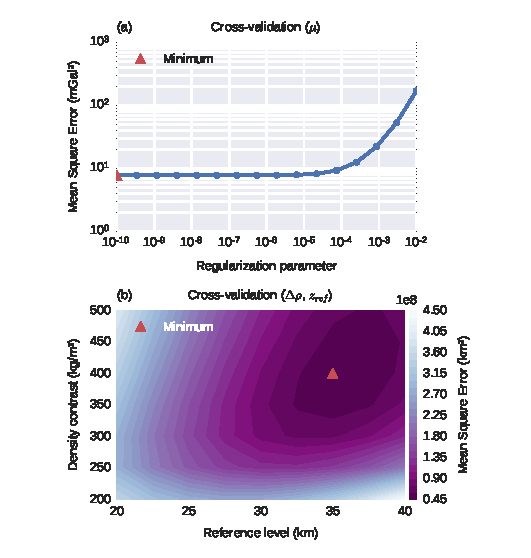
\includegraphics{figures/south-america-cv}
    \caption{
        Cross-validation results for the South American Moho inversion.
        (a) Cross-validation to determine the regularization parameter $\mu$
        (Eq.~\ref{eq:goalfunction}).
        The minimum Mean Square Error (Eq.~\ref{eq:msemu}),
        shown as a red triangle,
        corresponds to $\mu = 10^{-10}$.
        (b) Cross-validation to determine
        the reference level ($z_{ref}$) and the density-contrast ($\Delta\rho$).
        The colored contours represent
        the Mean Square Error (Eq.~\ref{eq:msehyper}).
        The minimum (red triangle) is found at $z_{ref} = 35\ km$
        and $\Delta\rho = 400\ kg/m^3$.
    }
    \label{fig:sam-cv}
\end{figure}

\begin{figure*}
    \centering
    
\includegraphics[width=\textwidth]{figures/south-america-moho}
    \caption{
        Inversion results for the South American Moho.
        (a) The estimated Moho depth of South America.
        (b) Differences between the seismological depths of
        \citet{assumpcao2012} and our gravity-derived estimate shown in (a).
        The inset in (b) shows a histogram of the differences along with their
        calculated mean and standard deviation (std).
    }
    \label{fig:sam-moho}
\end{figure*}

\begin{figure}
    \centering
    \includegraphics{figures/south-america-residuals}
    \caption{
        Residuals for the South American Moho inversion.
        The residuals are the observed data in Fig.~\ref{fig:sam-data}a
        minus the data predicted by the estimate in Fig.~\ref{fig:sam-moho}a.
        Shown as (a) a map and (b) a histogram with the calculated mean and
        standard deviation.
        (c) The value of the goal function (Eq.~\ref{eq:goalfunction})
        per Gauss-Newton iteration showing the convergence of the algorithm.
        Note that the y-axis is in logarithmic scale.
    }
    \label{fig:sam-residuals}
\end{figure}


\lipsum[1-7]



%%%%%%%%%%%%%%%%%%%%%%%%%%%%%%%%%%%%%%%%%%%%%%%%%%%%%%%%%%%%%%%%%%%%%%%%%%%%%%%
\section{Conclusions}

\lipsum[1-7]

%%%%%%%%%%%%%%%%%%%%%%%%%%%%%%%%%%%%%%%%%%%%%%%%%%%%%%%%%%%%%%%%%%%%%%%%%%%%%%%
\section{Acknowledgments}

The authors are indebted to the developers and maintainers of the open-source
software without which this work would not have been possible.

\bibliographystyle{gji}
\bibliography{biblio}

\end{document}
